\documentclass[c_worksheet.tex]{subfiles}

\begin{document}
	
\chapter{Arrays} 

Mit \emph{Arrays} lassen sich Daten ordentlich in einem Paket, wie eine Art Liste verwalten. \emph{Arrays} werden vielfach eingesetzt und sind eigentlich unumgänglich wenn man etwas aufwendigeres programmiert.

Man kann sich \emph{Arrays} wie eine Liste, in der nur Dinge des gleichen \emph{Types} drin stehen. Man kann auf jedes einzelne dieser Elemente zugreifen. Im Gegensatz zu den meisten anderen modernen Programmiersprachen, wissen \emph{Arrays} in \textbf{C} nicht wie lange diese sind. Darauf muss man beim schreiben eines Programms also selbst Acht geben und die Länge, gegebenen Falls in einer Variable speichern.

\begin{figure}[h]
\center
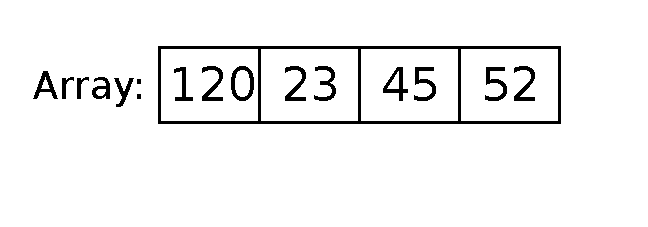
\includegraphics[width=0.7\textwidth]{Grafiken/Arrays/array.pdf} 
\end{figure}

\emph{Arrays} liegen im Speicher in einem einzigen Block hintereinander. Erzeugt man ein Array erhält man einen \emph{Pointer} auf das aller erste Element. Dieser \emph{Pointer} hat einen gewissen Typ, z.B. Interger, Float oder auch Character und weiß wie groß dieser ist. Auf einem 64Bit System ist ein Interger z.B. 4Byte groß.

Mit \emph{Pointer Arithmetik} kann man also die anderen Elemente des \emph{Arrays} erreichen in dem man im Adressbereich weiterspringt.

\begin{figure}[h]
\center	
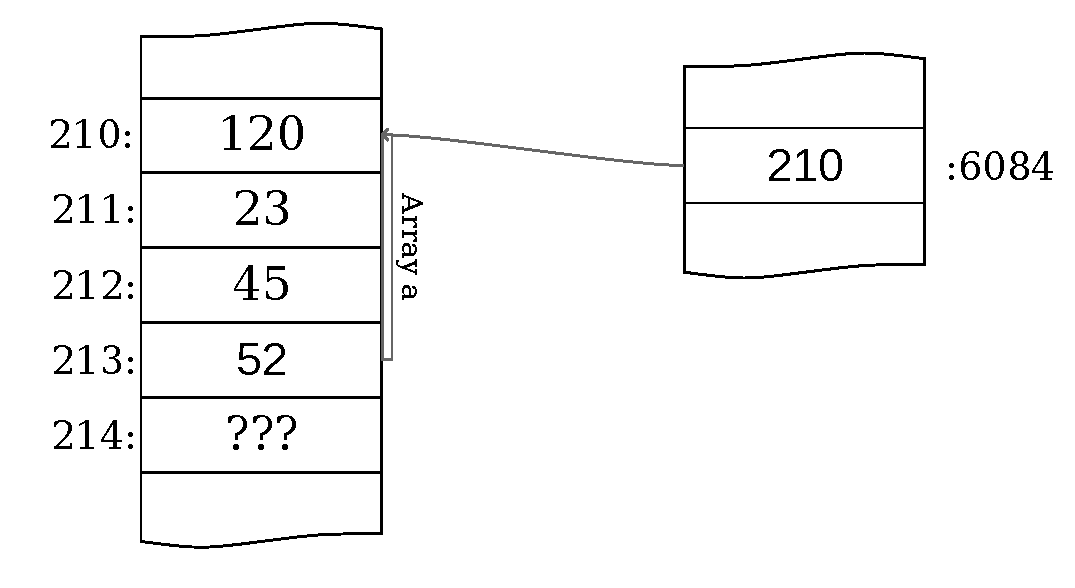
\includegraphics[width=0.8\textwidth]{Grafiken/Arrays/array_im_speicher.pdf} 
\end{figure}

\section{Initialisierung und die Grundlagen} 

\begin{lstlisting}
<Typ> <Arrayname> [ <Groesse> ]:
\end{lstlisting}

Die Initialisierung erfolgt also exakt wie bei einer normalen Variablen. Dazu muss aber noch eine Größe des Arrays angeben. Dabei werden im Speicher 4 aneinanderhängen 1 Byte große (da \emph{Character}) Blöcke frei geräumt und für das Programm reserviert (alloziert).

Man kann das \emph{Array} genau wie Variablen, schon bei der Initialisierung direkt mit Werte belegen.

\begin{lstlisting}
<Typ> <Arrayname> [ <Groesse> ] = { <Element1>, ... , <ElementN>};
\end{lstlisting}

Im folgenden gehen wir vom dem in der vorherigen Grafik dargestellten Szenario aus.

\lstinputlisting[firstline=1, lastline=2]{CodeSnippets/Arrays/array_initialisierung.c} 

Wenn man einen \emph{Pointer} auf a setz, kann man mit \emph{Pointer Arithmetik} auf die anderen Elemente zugreifen. Der \emph{Pointer} wird direkt auf a gesetzt, bekommt also den Wert der dort steht. Dieser ist lediglich die Adresse des ersten Elements, da a selbst auch nur ein \emph{Pointer} auf das erste Element ist.

\lstinputlisting[firstline=4, lastline=10]{CodeSnippets/Arrays/array_initialisierung.c} 

Mit dem +1 springt man im Adressbereich um eine \textbf{Typgröße} weiter. Da es sich in diesem Fall um ein \emph{Array} von \emph{Charactern} handelt, ist dies immer genau \textbf{1 Byte}. Wäre das ein \emph{Array} von \emph{Integern}, würde der \emph{Pointer} immer um \textbf{4 Byte} weiterspringen.

Man kann auch ohne Probleme aus dem Array heraus springen. Allerdings kann man unmöglich wissen, was an dieser Stelle im Speicher stehen wird.

\lstinputlisting[firstline=12, lastline=12]{CodeSnippets/Arrays/array_initialisierung.c} 

Auf dieser Art kann man natürlich auch den Inhalt des \emph{Arrays} verändern.

\lstinputlisting[firstline=14, lastline=15]{CodeSnippets/Arrays/array_initialisierung.c} 

\section{Elementzugriff} 


Damit man nicht immer mit \emph{Pointern} hantieren muss, wurde eine Syntax eingeführt, die den Elementzugriff erheblich erleichtert und einfacher macht.

Der Zugriff erfolgt dabei ähnlich wie die Initialisierung: über \textbf{eckige Klammern}. Dabei gilt es zu beachten, dass das erste Element eines \emph{Arrays} mit \textbf{0} indiziert ist. Ein \emph{Array} mit 4 Elementen hat also einen \emph{Indexbereich} von 0-3.

\begin{lstlisting}
<Arrayname> [ <Index> ]
\end{lstlisting}

Vergleicht man das ganze mit dem Zugriff über \emph{Pointer} sieht man auch, wieso der \emph{Index} bei \textbf{0} beginnt.

\lstinputlisting{CodeSnippets/Arrays/Elementzugriff.c} 

So kann man sehr einfach Werte eines \emph{Arrays} auslesen oder diese verändern.

Diese Syntax ist die gängige und am meisten genutzte Syntax. Sie ist leicht zu verstehen und erspart einem den direkten Kontakt mit \emph{Pointern}.


\section{Arrays und Schleifen}

Eine typische Aufgabe ist es mit Schleifen über \emph{Arrays} zu \emph{iterieren} bzw. durch diese zu laufen. Egal ob zum auslesen oder um Werte dort hinein zu schreiben. Das geht mit einer gewöhnlichen \emph{for Schleife} sehr leicht und ist eine typische Anwendung, wie sie ständig vorkommt.

Folgender Code gibt alle Elemente eines \emph{Arrays} a aus.

\lstinputlisting{CodeSnippets/Arrays/array_for1.c} 

Folgender Code setzt die aufsteigende Zahlenfolge in ein Array

\lstinputlisting{CodeSnippets/Arrays/array_for2.c} 

Das Array sähe danach so aus:

\begin{center}
``\textit{[1, 2, 3, 4, 5, 6, 7, 8, ...]}'' 
\end{center}

Mit einer \emph{for Schleife} kann man also sehr einfach und elegant über ein \emph{Array} iterieren. Dabei muss man lediglich die Länge des Arrays kennen.


\section{Arrays und Funktion} 

Ein \emph{Array} als Funktionsparameter zu übergeben ist nicht ganz so einfach wie bei einer gewöhnlichen Variable. Es gibt dazu prinzipiell 3 Methoden, wovon zwei sich aber sehr ähnlich sind.

\subsection{Paramter als Array} 

Man kann einmal als Paramter wirklich direkt die Arraysyntax angeben. Das geht einmal mit Länge und einmal ohne Länge. Gibt man das ganze mit Länge an, kann man wirklich nur \emph{Arrays} mit dieser Länge der \emph{Funktion} übergeben. Das ist eine starke Einschränkung und sollte meist vermieden werden.

\lstinputlisting{CodeSnippets/Arrays/array_function_parameter1.c}

Das ganze ginge natürlich auch mit der Funktionssignatur \lstinline$ int sum(int a[])$, dann könnte man auch Arrays übergeben, die länger als 10 sind. Jedoch kennt man die Länge dann nicht. Das kann aber sehr einfach wie folgt gelöst werden.
 
\lstinputlisting{CodeSnippets/Arrays/array_function_parameter2.c}

\subsection{Paramter als Pointer}

Die andere Methode ist über \emph{Pointer}. Wie am Anfang besprochen, ist ein \emph{Array} nichts anderes als ein \emph{Pointer} auf das erste Element des Arrays. Also kann man als Parameter in der Funktion einfach einen \emph{Pointer} des entsprechenden \emph{Datentyps} angeben.

\lstinputlisting{CodeSnippets/Arrays/array_function_parameter_pointer.c} 


\end{document}